\documentclass[11pt, a4paper]{article}
\usepackage[utf8]{inputenc}
\usepackage[spanish, es-tabla, es-nodecimaldot]{babel}
\usepackage{sansmathfonts}				% Sans Serif equations
\renewcommand*\familydefault{\sfdefault} 		% Sans Serif as default font
\usepackage[a4paper, 					% Page Layout
                     %showframe,				% This shows the frame
                     includehead,
                     footskip=7mm, headsep=6mm, headheight=4.8mm,
                     top=25mm, bottom=25mm, left=25mm, right=25mm]{geometry}
\RequirePackage{caption} 				% Caption customization
\captionsetup{justification=centerlast,font=small,labelfont=sc,margin=1cm}
\usepackage{hyperref}
\hypersetup{
    colorlinks=true,
    linkcolor=blue,
    filecolor=magenta,      
    urlcolor=blue,
    citecolor=blue,    
}
\usepackage{fancyhdr}
\fancyhead{}
\lhead{A la izquierda}
\rhead{\framebox{A la derecha con borde}}
\fancyfoot{}
\rfoot{\thepage}
\pagestyle{fancy}
\renewcommand{\headrulewidth}{0pt}
\renewcommand{\footrulewidth}{0.5pt}

\usepackage{array}
\newcommand{\PreserveBackslash}[1]{\let\temp=\\#1\let\\=\temp}
\newcolumntype{C}[1]{>{\PreserveBackslash\centering}p{#1}}
\newcolumntype{R}[1]{>{\PreserveBackslash\raggedleft}p{#1}}
\newcolumntype{L}[1]{>{\PreserveBackslash\raggedright}p{#1}}

\usepackage{tikz}
\usetikzlibrary{babel}

\usepackage{amsmath}
\usepackage{bm}


\title{TikZ}
\author{Dr. Ing. Pablo Cossutta}
\date{2019}

\begin{document}
\maketitle
\section{Dibujos en TikZ}
En la Fig. \ref{fig1} se observa un diagrama realizado en tikz.
%
\begin{figure}[h]%
	\centering
	\begin{tikzpicture}
		\tikzstyle{every node}=[font=\footnotesize]	
		\tikzstyle{base} = [draw, align=center, line width=0.25mm, fill={rgb,255:red,204; green,255; blue,204}, minimum width=2cm, minimum height=1.25cm]	
		\tikzstyle{blank} = [align=center, inner sep=0pt, outer sep=0pt]	
		\tikzstyle{block} = [draw, rounded corners=0.1cm, align=center, line width=0.25mm, fill={rgb,255:red,209; green,225; blue,243}, minimum width=2cm, minimum height=2cm]	
		\tikzstyle{flecha} = [->, line width=0.25mm, >=latex]
		\tikzstyle{linea} = [line width=0.25mm, >=latex]
		\tikzstyle{meas} = [draw, rectangle, densely dashed, minimum width=0.2cm, minimum height=0.6cm]
		\tikzstyle{circulo} = [circle,fill=black,inner sep=0pt,minimum size=3pt]	
		
		\draw(-2.75cm,0.5cm) node[blank, label=left:$\bm{x^*}_k$](input){};
		\draw(-1cm, 0.5cm) node[block, minimum height=1cm](extra){Extrapolación};
		\draw [flecha] (input) -- (extra);
		\draw [flecha] (extra.east) --++ (0.92cm,0) node[midway,blank, label=above:$\bm{x^*}_{k+n}$]{};
		
		\draw (2cm,0) node[block](min){Minimización\\de la función\\de costo};
		\draw (2cm,-2.5cm) node[block](pred){Modelo\\de\\predicción};
		\draw (5.5cm,0) node[base, minimum height=1.25cm, fill={rgb,255:red,255; green,204; blue,204}](conv){Convertidor};
		\draw (8.5cm,0) node[base](load){Carga};
		\draw (5.5cm,-2.5cm) node[block, minimum height=1.25cm](med){Mediciones};
		\draw [flecha] (min.east) -- (conv.west) node[midway, label=above:$\bm{s}^{opt}$]{};
		\draw [flecha] (conv.east) -- (load);
		\draw [flecha] (conv.south) -- (med.north);
		\draw [flecha] (load.south) |- (med.east);
		\draw[flecha] (med.west) -- (pred.east) node[midway, blank, label=above:$\bm{x}_k$]{};
		\draw[flecha] (pred.west) -| (0.5cm,-0.5cm) node[blank, label=left:$\bm{x}_{k+n}$]{} --++ (0.49cm, 0);
		\draw[linea, dashed] (-2.33cm,1.25cm) --++ (5.6cm,0cm) --++ (0cm,-5cm) 
		   --++(-5.6cm,0cm) -- cycle;
		\draw (-0.45cm, -3.75cm) node[anchor=south east, align=center]{Controlador\\FCS-MPC};
	\end{tikzpicture}%
	\caption{Diagrama realizado en TikZ}
	\label{fig1}
\end{figure}

La Fig. \ref{fig2} se incluye desde el pdf realizado en \textit{circuitikz}. 

\vspace{1em}

El comando \textbackslash label va siempre despues de \textbackslash caption.
\begin{figure}[h!]
	\centering
	
\includegraphics[page=2]{../5-circuitikz/circuitikz.pdf}
	\caption{Realizada en modo standalone}
	\label{fig2}
\end{figure}

\newpage
La Fig. \ref{fig3} se incluye desde TikZ para poder realizar anotaciones sobre la misma. 
\begin{figure}[h]
	\centering
	\begin{tikzpicture}[image/.style={anchor=south west,inner sep=0,outer sep=0}]
		\tikzstyle{every node}=[font=\footnotesize]	
		\tikzstyle{block} = [align=center]	
		\tikzstyle{flecha} = [->, line width=0.25mm, >=latex]
		\node[anchor=south west,inner sep=0, outer sep=0] (image) at (0,0) {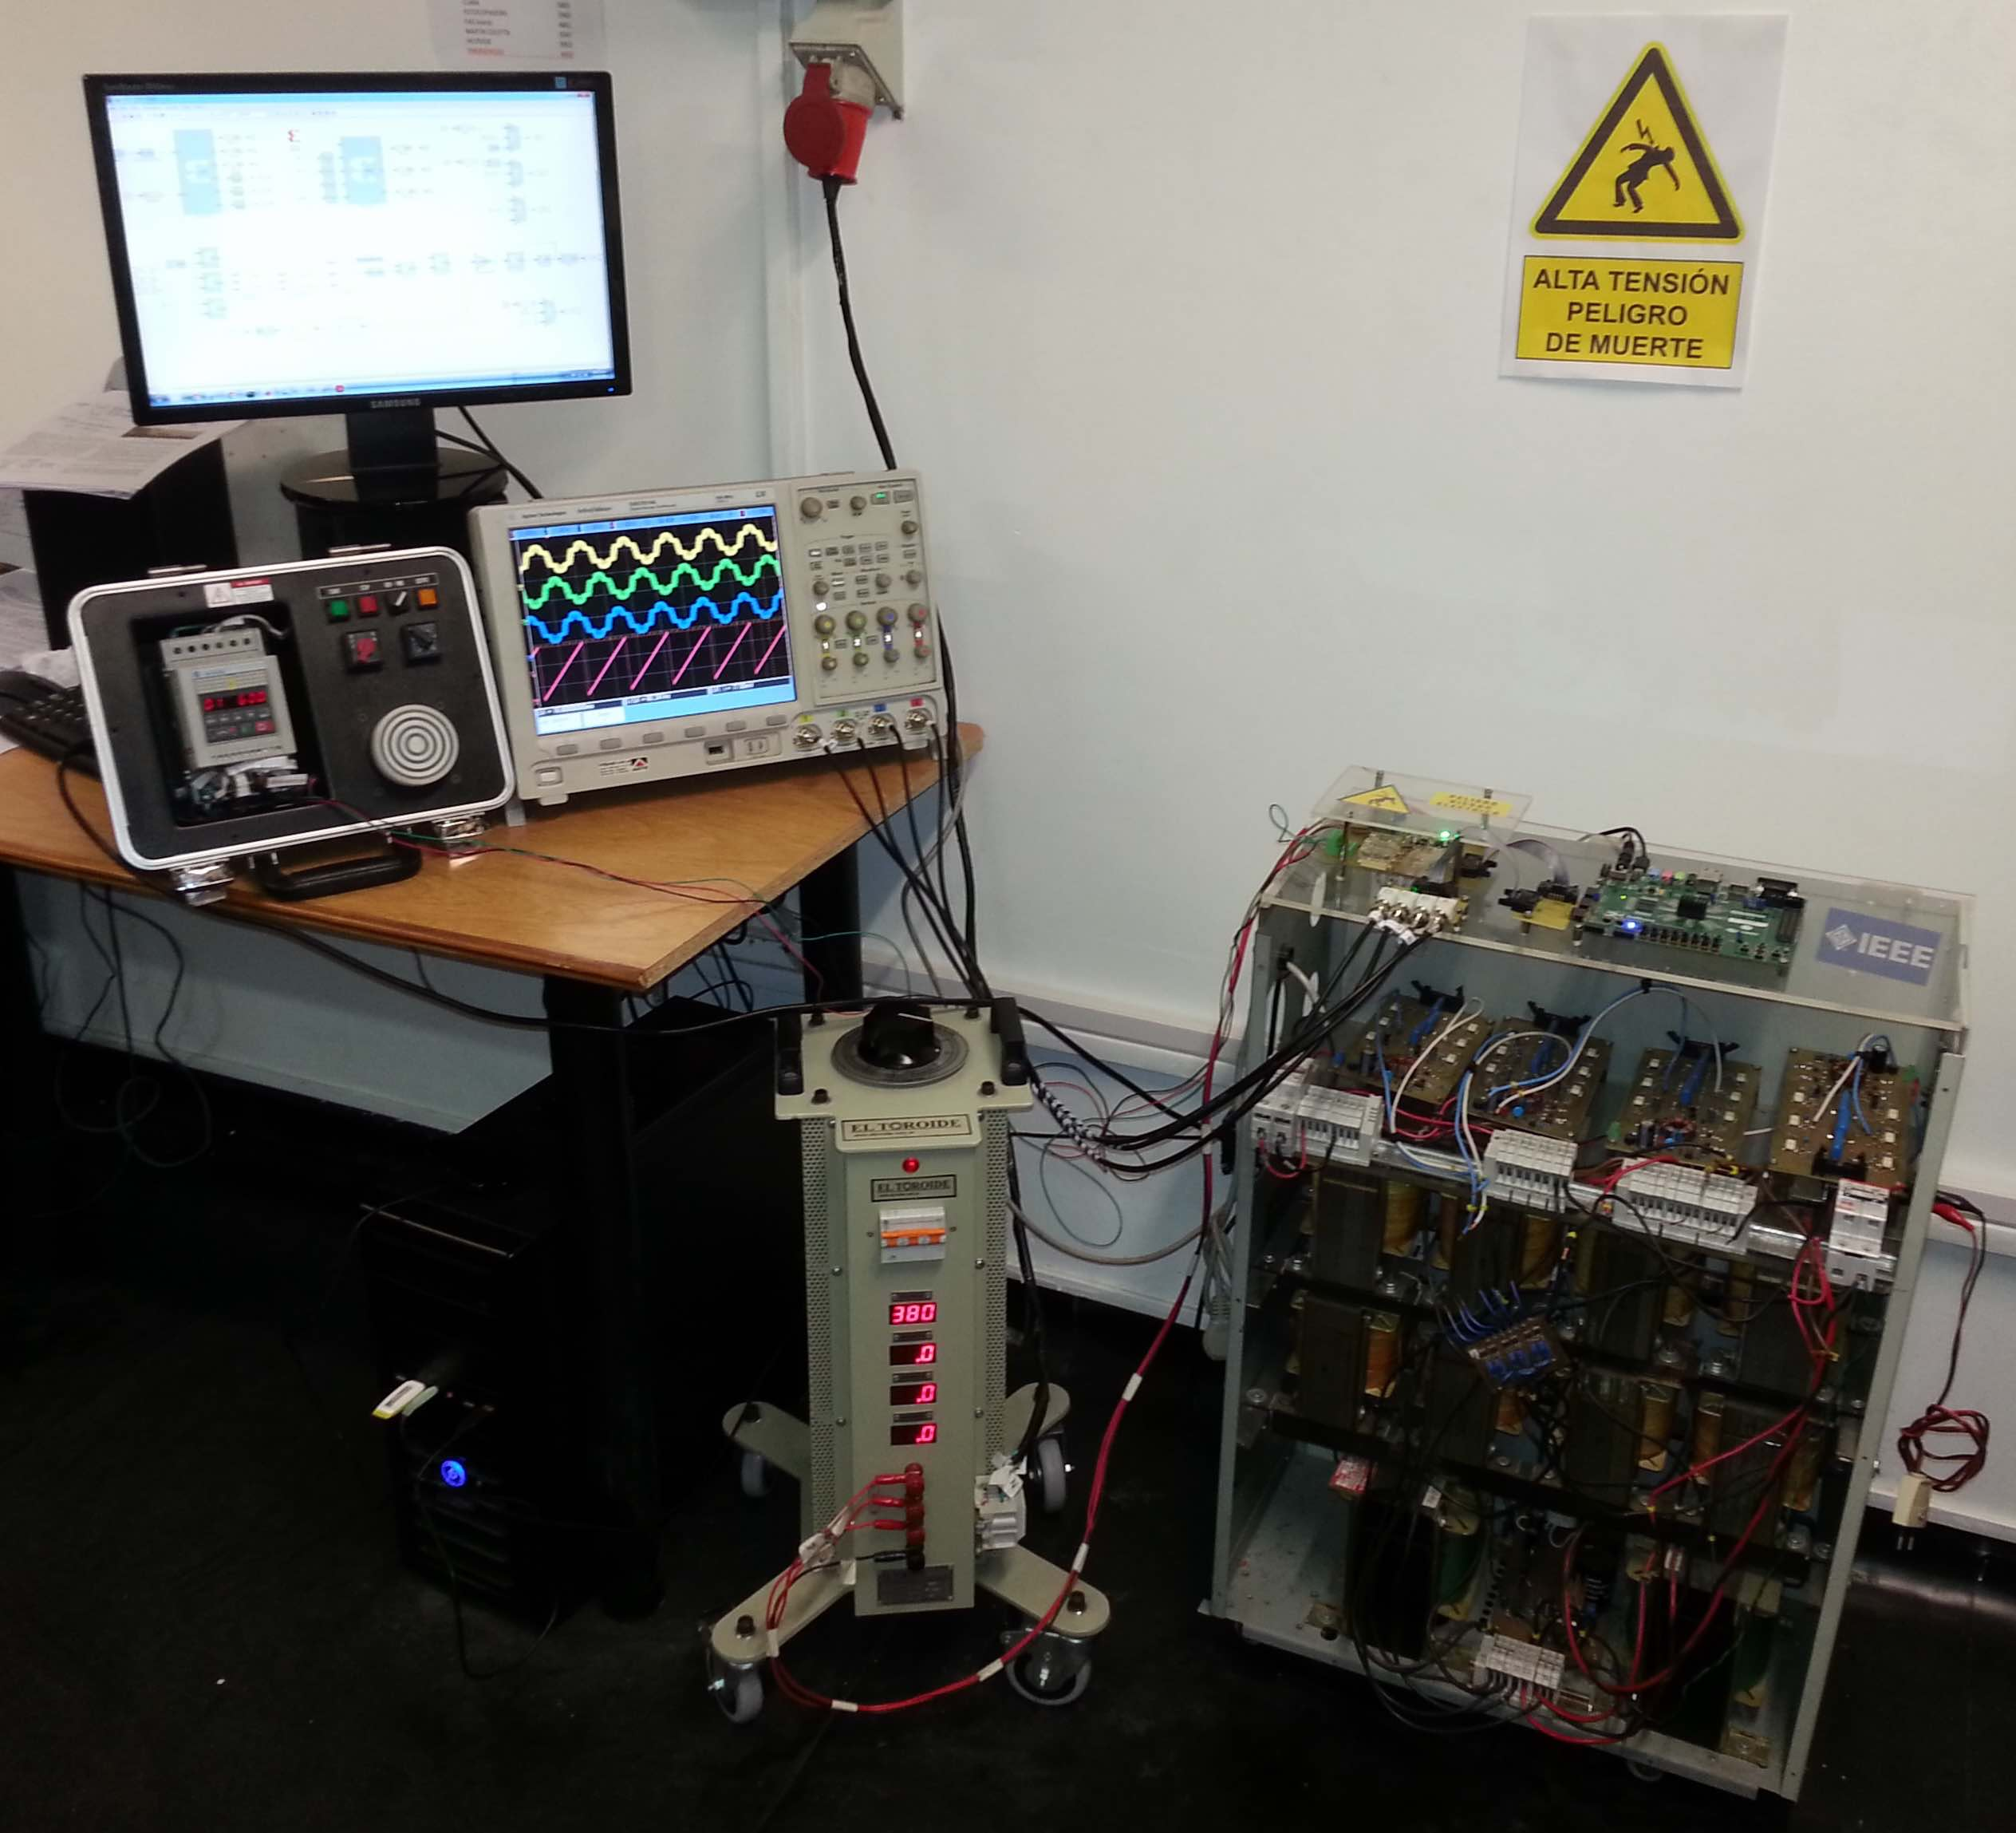
\includegraphics[width=9cm]{fig3.jpg}};
		\begin{scope}[x={(image.south east)},y={(image.north west)}]
		        %\draw[help lines,xstep=.1,ystep=.1] (0,0) grid (1,1);
		        %\foreach \x in {0,1,...,9} { \node [anchor=north] at (\x/10,0) {0.\x}; }
		        %\foreach \y in {0,1,...,9} { \node [anchor=east] at (0,\y/10) {0.\y}; }		        
			\node at (0.61, 0.95) [block](a){MATLAB Simulink};
			\node at (0.61, 0.85) [block](b){Convertidor\\Industrial};
			\node at (0.61, 0.73) [block](c){Autotransformador\\Variable};
			\node at (0.72, 0.62) [block]{Interfaz\\Analógica};
			\node at (0.88, 0.57) [block]{FPGA};
			\draw [flecha] (a.west) -- (0.31,0.87);
			\draw [flecha] (b.west) -- (0.23,0.695);
			\draw [flecha] (c.south) -- (0.5,0.48);
		\end{scope}
	\end{tikzpicture}%
	\caption{Figura con anotaciones en TikZ}
	\label{fig3}
\end{figure}

Finalmente, la Fig. \ref{fig4} denota el uso del parámetro \textit{trim} del comando \textbackslash includegraphics.

\begin{figure}[h]
	\centering
	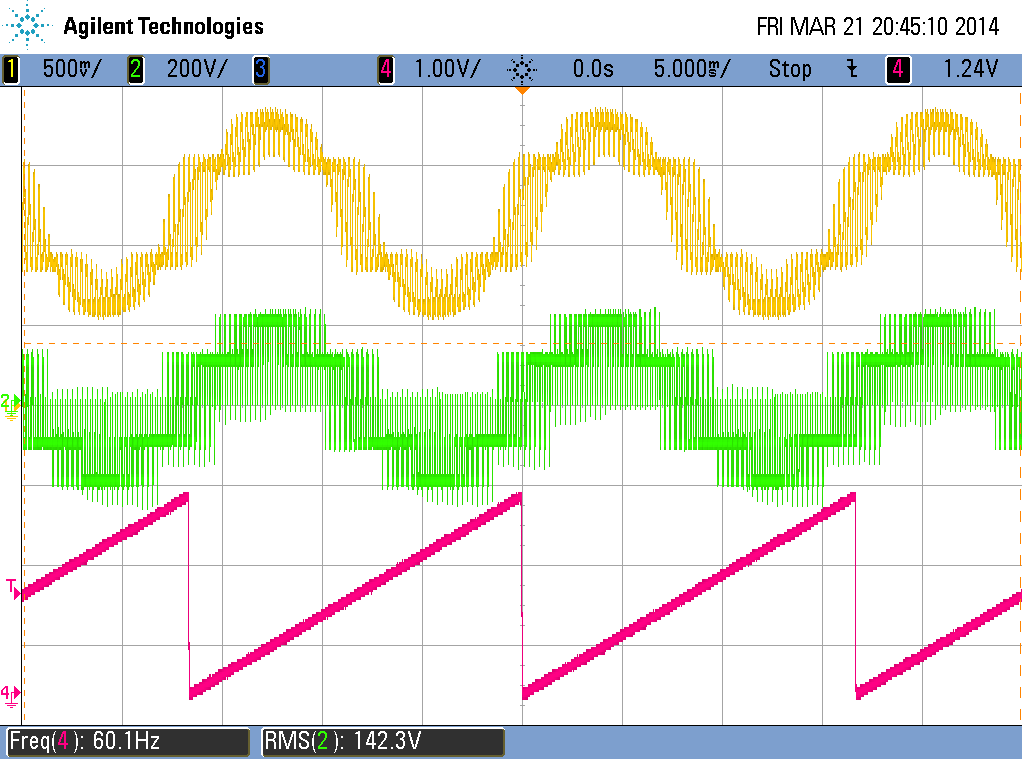
\includegraphics[trim={0 0 0 1.35cm}, clip, width=10cm]{fig4.png}
	\caption{Utilización del parámetro \textit{trim} de \textbackslash includegraphics}
	\label{fig4}
\end{figure}

\section{Herramientas}
Existe una herramienta online \href{https://www.mathcha.io}{Matcha} que simplifica la realización de diagramas en TikZ.

En \LaTeX \space podemos hacer cosas raras en latex como
\vfill
\begin{center}
	Poner esto al medio de lo que queda de espacio
\end{center}
\vfill
Poner esto abajo \hfill y \hfill Poner esto al final.
\end{document}
